\documentclass[a4paper,10pt,oneside]{article}
\usepackage{graphicx}
\usepackage{color}
\usepackage{url}
\usepackage{subfigure}
\usepackage[utf8]{inputenc}
\usepackage[T1]{fontenc}
\usepackage{tgpagella}
%\usepackage[scale=0.9]{tgcursor}
%\usepackage[scale=0.9]{tgheros}
\usepackage{xstring}

\newcommand{\myscale}{0.74}
\newcommand{\vect}[1]{\boldsymbol{#1}}
\newcommand{\code}[1]{\texttt{\StrSubstitute{#1}{.}{.\.}}}
\def\.{\discretionary{}{}{}}
\newcommand{\jmodule}[1]{\texttt{\textit{#1}}}

\setlength{\hoffset}{-1in} %left margin will be 0, as hoffset is by default 1inch
\setlength{\voffset}{-1in} %analogous voffset
\setlength{\oddsidemargin}{1.5cm}
\setlength{\evensidemargin}{1.5cm}
\setlength{\topmargin}{1.5cm}
\setlength{\textheight}{24cm}
\setlength{\textwidth}{18cm}

\def\mftitle{jInfer ProjectType Module Description}
\def\mfauthor{Michal Klempa, Mário Mikula, Robert Smetana, Michal Švirec, Matej Vitásek}
\def\mfadvisor{RNDr. Irena Mlýnková, Ph.D., Martin Nečaský, Ph.D.}
\def\mfplacedate{Praha, 2011}
\title{\bf\mftitle}
\author{\mfauthor \\ Advisors: \mfadvisor}
\date{\mfplacedate}

\ifx\pdfoutput\undefined\relax\else\pdfinfo{ /Title (\mftitle) /Author (\mfauthor) /Creator (PDFLaTeX) } \fi

\begin{document}
\maketitle
\noindent Target audience: developers willing to extend jInfer, specifically extend jInfer project structure.

\noindent \begin{tabular}{|l|l|} \hline
Responsible developer: & Michal Švirec \\ \hline
Required tokens:       & cz.cuni.mff.ksi.jinfer.base.interfaces.inference.IGGenerator \\
 & cz.cuni.mff.ksi.jinfer.base.interfaces.inference.SchemaGenerator \\
 & cz.cuni.mff.ksi.jinfer.base.interfaces.inference.Simplifier \\
 & org.openide.windows.IOProvider \\ \hline
Provided tokens:       & none \\ \hline
Module dependencies:   & Base \\
	& Runner \\ \hline
Public packages:       & cz.cuni.mff.ksi.jinfer.projecttype.actions \\ \hline
\end{tabular}

\section{Introduction}

\jmodule{ProjectType} is the module representing a jInfer project in the NB platform, grouping input/output files that belong to one specific inference. Each jInfer project also allows the user to set properties specific for this inference.\\

\begin{figure}
	\subfigure[Legend: Rectangle is folder, Rounded rectangle is file.] {
		\centering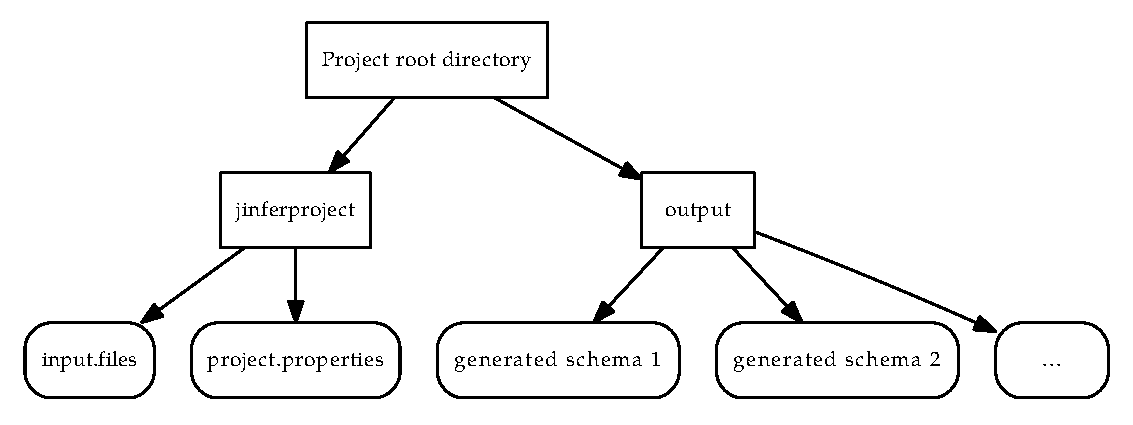
\includegraphics[scale=\myscale]{project_dir_structure}
	}
	\caption{Project directory structure.} \label{dir-structure}
\end{figure}

For each jInfer project a specific directory structure in the filesystem describing this project is created. This structure is described in figure \ref{dir-structure}. A folder in the filesystem is considered to be jInfer project folder if it contains a \emph{jinferproject} subfolder. This folder contains two files: \emph{project.properties}, where all properties set for that particular project are stored. The second file is \emph{input.files} which is an XML file filled with paths to files selected as particular project input (structure of this file is described in section \ref{input.files}). \emph{output} subfolder contains schema files which were generated by jInfer inference runs.

\section{Structure}

Structure of \jmodule{ProjectType} can be divided into the following five main parts.
\begin{itemize}
	\item Base classes - Classes providing core functionality like project creation and definitions of operations like move, delete, copy etc. All the base classes are contained in the \code{cz.\.cuni.\.mff.\.ksi.\.jinfer.\.projecttype} package.
	\item Visualization classes - These classes create tree structure of jInfer project in NBP Projects view and are contained in the \code{cz.\.cuni.\.mff.\.ksi.\.jinfer.\.projecttype.\.nodes}.
	\item Actions - Classes from \code{cz.\.cuni.\.mff.\.ksi.\.jinfer.\.projecttype.\.actions} package that provide actions allowing adding input files into the project, removing input files, or running the inference on the project.
	\item Properties - Classes responsible for creation of project properties window with properties category tree. These are located in \code{cz.\.cuni.\.mff.\.ksi.\.jinfer.\.projecttype.\.properties} package.
	\item Project wizard - Classes representing new project creation through a project wizard from \code{cz.\.cuni.\.mff.\.ksi.\.jinfer.\.projecttype.\.sample} package.
\end{itemize}

\subsection{Base classes}

This section describes classes needed for jInfer project creation and its integration into the NBP. The two main classes representing a jInfer project type are \code{JInferProjectFactory} and \code{JInferProject}.

\subsubsection{JInferProjectFactory}

\code{JInferProjectFactory} is a factory class implementing \code{ProjectFactory} interface provided by NBP. This class is responsible for loading/saving the jInfer project from/to the filesystem and also determining if a folder in filesystem is of jInfer project type (= contains \emph{jinferproject} subfolder). For this purpose, class has three methods: \code{isProject()}, \code{save()} and \code{load()}. When jInfer project is loaded from the filesystem, \code{JInferProjectFactory} creates new instance of \code{JInferProject} passing path to project folder as a constructor parameter. When \code{save()} method is invoked, all the project properties are saved in \emph{project.properties} file and paths to input files are saved into \emph{input.files}.

\subsubsection{JInferProject}

\code{JinferProject} class implements the \code{Project} interface from NBP and represents an in-memory representation of a jInfer project. Inner structure of this class is very simple, interface specifies only two methods: \code{getProjectDirectory()} and \code{getLookup()}. All the extensibility of a project type is done by the \emph{Lookup} functionality of NBP. Project lookup contains properties, \code{Input} class (encapsulating input files), class creating output files, class building project tree in the Projects view, etc.

\subsubsection{InputFiles}\label{input.files}

\code{InputFiles} is a utility class that stores/loads input file paths into/from the \emph{input.files} XML file. For this purpose, \code{InputFiles} uses \emph{JAXB} \cite{JAXB} framework to unmarshall/marshall XML file into/from Java content objects. XML structure of \emph{input.files} is very simple, \emph{jinferinput} is the root element under which are \emph{documents}, \emph{schemas} and \emph{queries} elements. Each of this elements may have none or more \emph{file} elements with string attribute \emph{loc} that contains the absolute path to the input file.\\

\noindent Example of \emph{input.files} follows.
\begin{verbatim}
	<?xml version="1.0" encoding="UTF-8" standalone="yes"?>
	<jinferinput>
	    <xml>
	        <file loc="/home/user/example1.xml"/>
	        <file loc="/home/user/example2.xml"/>
	    </xml>
	    <schemas>
	        <file loc="/home/user/example.dtd"/>
	    </schemas>
	    </queries/>
	</jinferinput>
\end{verbatim}

\subsection{Visualization classes}

\begin{figure}
	\centering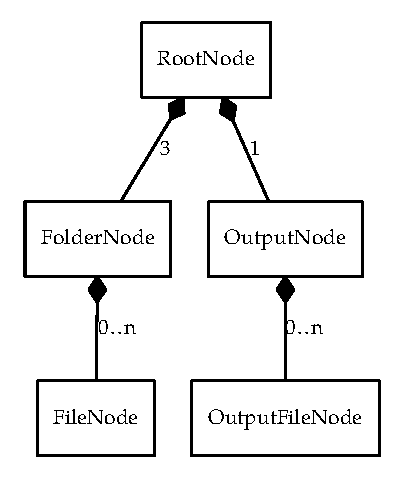
\includegraphics[scale=\myscale]{node_structure}
	\caption{Project nodes structure.} \label{node-structure}
\end{figure}

Each jInfer project in NBP is open after its creation in the Projects view and has tree structure where each node is represented by a NBP \code{Node} class. This structure in jInfer project type is provided by the \code{JInferLogicalView} class implementing \code{LogicalViewProvider} interface from NBP and is available through the \code{JInferProject} lookup. This class has one important method: \code{createLogicalView()} returning an instance of \code{RootNode} class. Simple class structure is described in figure \ref{node-structure}.\\

\code{RootNode} extends NBP \code{AbstractNode} class which is a basic implementation of NBP \code{Node}. This node contains four children nodes: three for input files (Document, Schema and Query) and one for output files generated by the inference (Output). Root node also offers actions for adding input files, inference running and standard project actions like delete or move/rename project.\\

Each of the \emph{input} nodes is represented by a \code{FolderNode} class and contains \emph{input file} nodes (represented by a \code{FileNode} class) representing files added to the jInfer project. Notice that these \emph{input file} nodes represent existing files in the filesystem and are not copied to the project folder structure. Because of this, if you delete these nodes from project tree, files in the filesystem are not affected.\\

\code{OutputNode} class represents an \emph{Output} node in jInfer project type tree and is slightly different from \emph{input} nodes, because it refers to \emph{output} subfolder in project filesystem hierarchy. In other words, files contained in this folder are shown as subnodes in \emph{Output} node in project tree. These subnodes are represented by \code{OutputFileNode} class. Unlike \emph{input file} nodes, if you delete \emph{output file} node under the \emph{Output} node, file represented by this node is deleted from filesystem too.

\subsection{Actions}

Each node in jInfer project tree hierarchy contains a set of actions available from its context menu. Besides standard NBP actions for root node or file node, jInfer project type introduces its own actions. These actions can be divided into three groups: actions for \emph{root} node, actions for \emph{input folder} nodes and one action for \emph{input/output file} nodes implemented by \code{ValidateAction} class. All classes implementing a jInfer project action extend standard java \code{javax.\.swing.\.AbstractAction} class besides \code{ValidateAction} class which is described in \ref{validate-action}.\\

\subsubsection{Root node actions}

This group contains two actions: an action that allows adding input files into \emph{input folder} nodes (implemented by \code{FilesAddAction} class). Second one is slightly different, because it implements functionality for an item that already exists in context menu - Run action.\\

After invoking the first of the two actions, a file chooser dialog is open. Its file filter is set according to available classes implementing \code{Processor} interface registered in jInfer with \code{ServiceProvider}. After selecting file(s) in dialog, these files are inserted into the particular \emph{input folder} node according to mapping of their file extensions to folder type retrieved from \code{Processor} classes. If no mapping for some extension exists, this file is inserted into a default folder defined in \emph{Miscellaneous} properties category (section \ref{pref}).\\

Run action, available from root node context menu, is also present in NBP toolbar as a \emph{Run} button and in jInfer Welcome window. This action is implemented in \code{RunAction} class and simply invokes \jmodule{Runner}'s \code{run()} method, if no other inference is already running. Otherwise an information dialog pops up, informing about the already running inference. This check is done invoking the \code{setActiveProject()} from \code{RunningProject} class (section \ref{running-project}).

\subsubsection{Input folder node actions}

Two actions belong to this group: action for adding input files into \emph{input folder} node (\code{FileAddAction} class) and action for deleting all input files in the \emph{input folder} node (\code{DeleteAllAction} class). \code{FileAddAction} class implements action which opens a file chooser dialog and adds the selected files into the particular \emph{input folder} node. \code{DeleteAllAction} class simply removes all input files previously added into that particular \emph{input folder} node.

\subsubsection{ValidateAction}\label{validate-action}

\code{ValidateAction} class implements action that allows documents and schema files to be validated against each other. Because of this, action is presented in context menu of document and schema files (its actual implementation is available for XML, DTD and XML Schema files). Unlike the other action classes, this extends NBP \code{NodeAction} class, which allows to enable/disable the action in context menu according to node selection. Action is enabled only if exactly one schema file and one or more XML files are selected at the same time. If the selected XML files are valid against selected schema, information dialog pops up, otherwise error dialog pops up and an error message describing the cause of non-validity of XML files against this schema is printed in \emph{validate} output window.\\

For the validation against XML Schema, we use standard Java validation API \cite{xml_validate}. Besides XML Schema, this API allows to validate XML also against \emph{Relax NG} and \emph{Schematron} schema. If you want to extend the functionality of one of these schemas, you need to set \code{schemaLanguage} local variable to appropriate \code{XMLConstant}. If you need to extend validation to some other type of schema, you can use DTD validation as an example.\\

For validation error handling the \code{JInferErrorHander} class is used. It extends \code{DefaultHandler} class and overrides its \code{error()} and \code{fatalError()} methods. In these methods an error message is created, which is consequently printed in validation \emph{output} window.

\subsection{Properties}

Each jInfer project has its associated properties window through which the user can change project-wide properties. This window is accessible through \emph{Properties} action in context menu of the project \emph{root} node. Properties window consists of category tree on the left side and properties pane on the right side. With each category in the tree, one properties pane is associated. Structure of the category tree consists of two types of categories: actual categories provided by some modules and \emph{virtual} categories. An actual category has its associated properties pane, which is displayed in the right side of the properties window. \emph{Virtual} category is displayed as a special information panel in the properties pane that provides information about count and names of modules which are children of this virtual category. Each actual category can have either virtual or actual categories as its children, but not both at a same time. On the other hand, a \emph{virtual} category can have only actual categories as its children. If a \emph{virtual} category has no children, this category is not displayed in the category tree.\\

A category in the properties window is represented by NBP \code{ProjectCustomizer.Category} class, properties pane is represented by \code{JPanel} class. Classes responsible for creation of this properties window are \code{JInferCustomizerProvider} and \code{JInferComponentProvider}. From jInfer module point of view the properties category is represented by \code{Properties\-Panel\-Provider} interface and associated properties pane by \code{AbstractPropertiesPanel} abstract class. How to use this interface and abstract class to create custom project properties category presented in jInfer project properties window is described in section \ref{properties_reg}.\\


\code{JInferComponentProvider} is a very simple class that extends \code{ProjectCustomizer.CategoryComponentProvider} class from NBP and its only method is \code{create()} which takes category as a parameter and returns properties pane. In the \code{JInferCustomizer\-Provider} class (which extends NBP \code{CustomizerProvider} class) is the core functionality of collecting categories (\code{PropertiesPanelProvider} interface) with associated properties panes (\code{AbstractPropertiesPanel} class) from all jInfer modules.\\

\subsubsection{Custom project properties category}\label{properties_reg}

As was written before, each jInfer project properties category is represented in jInfer modules by \code{PropertiesPanelProvider} interface. To create new category, this interface must be implemented and implementation must be annotated by the following code.
\begin{verbatim}
	@ServiceProvider(service = PropertiesPanelProvider.class)
\end{verbatim}

\noindent\code{PropertiesPanelProvider} interface provides the following methods:
\begin{itemize}
	\item getName() - Gets a programmatic name of this category.
	\item getDisplayName() - Gets a name of this category which will be displayed in properties window.
	\item getPriority() - Gets priority of this category, by which it is sorted among other sibling categories in the tree.
	\item getPanel(Properties) - Gets the \code{AbstractPropertiesPanel} instance representing the category \emph{properties pane}. The only parameter is an instance of \code{Properties} class holding stored properties for the \emph{properties pane}.
	\item getParent() - Getter for a programmatic name of category which is the parent of this category in the tree hierarchy.
	\item getSubCategories() - Gets a \code{List} of \code{VirtualCategoryPanel} instances representing virtual category children.
\end{itemize}


\noindent Example of the implemented \code{PropertiesPanelProvider}.

\begin{verbatim}
@ServiceProvider(service = PropertiesPanelProvider.class)
public class PropertiesPanelProviderImpl implements PropertiesPanelProvider {

  @Override
  public AbstractPropertiesPanel getPanel(Properties properties) {
    return new ExamplePropertiesPanel(properties);
  }

  @Override
  public String getName() {
    return "exampleCategoryID";
  }

  @Override
  public String getDisplayName() {
    return "Example category";
  }

  @Override
  public int getPriority() {
    return 1000;
  }

  @Override
  public String getParent() {
    return null;
  }

  @Override
  public List<VirtualCategoryPanel> getSubCategories() {
    List<VirtualCategoryPanel> result = new ArrayList<VirtualCategoryPanel>();
    result.add(new VirtualCategoryPanel("virtual_categoryID", "example virtual category",
            ModuleSelectionHelper.lookupImpls(IGGenerator.class)));

    return result;
  }
\end{verbatim}

\noindent\code{VirtualCategoryPanel} extends \code{JPanel}, its constructor has three parameters:
 \begin{itemize}
	\item \code{categoryId} - Programmatic name of the category or ID.
	\item \code{categoryName} - Human readable name of the category displayed in jInfer properties window.
	\item \code{modules} - \code{List<?\ extends NamedModule>} of modules that will be children of this virtual category.
\end{itemize}

To create properties pane associated with a custom category, class extending \code{AbstractPropertiesPanel} class must be implemented. As you can see from the class diagram in the Figure \ref{uml-properties}, this abstract class has a constructor with \code{Properties} parameter and two abstract methods, \code{store()} and \code{load()}, which must be implemented. Constructor gets a \code{Properties} instance as a parameter and saves it to \code{protected} field \code{properties}. This \code{Properties} instance is associated with jInfer project type \emph{lookup} and is used to store properties that are set in this panel.\\

Purpose of the method \code{store()} can be easily guessed from its name, it's used to store values that are set in \emph{properties pane} elements (text fields, checkboxes etc.) to the provided \emph{properties} field. On the other hand, \code{load()} method is used to populate \emph{properties pane} elements with already saved values in the \emph{properties}.

\noindent Example of the implemented \code{AbstractPropertiesPanel}.

\begin{verbatim}
public class ExamplePropertiesPanel extends AbstractPropertiesPanel {

  private JCheckBox checkBox;

  public ExamplePropertiesPanel(Properties properties) {
    super(properties);
    init();
  }

  public void init() {
    ...
    // initialize checkBox
    ...
  }

  @Override
  public void store() {
    properties.setProperty("some_property", Boolean.toString(checkBox.isSelected()));
  }

  @Override
  public void load() {
    checkBox.setSelected(Boolean.parseBoolean(properties.getProperty("some_property", "true")));
  }
}
\end{verbatim}

\begin{figure}
	\centering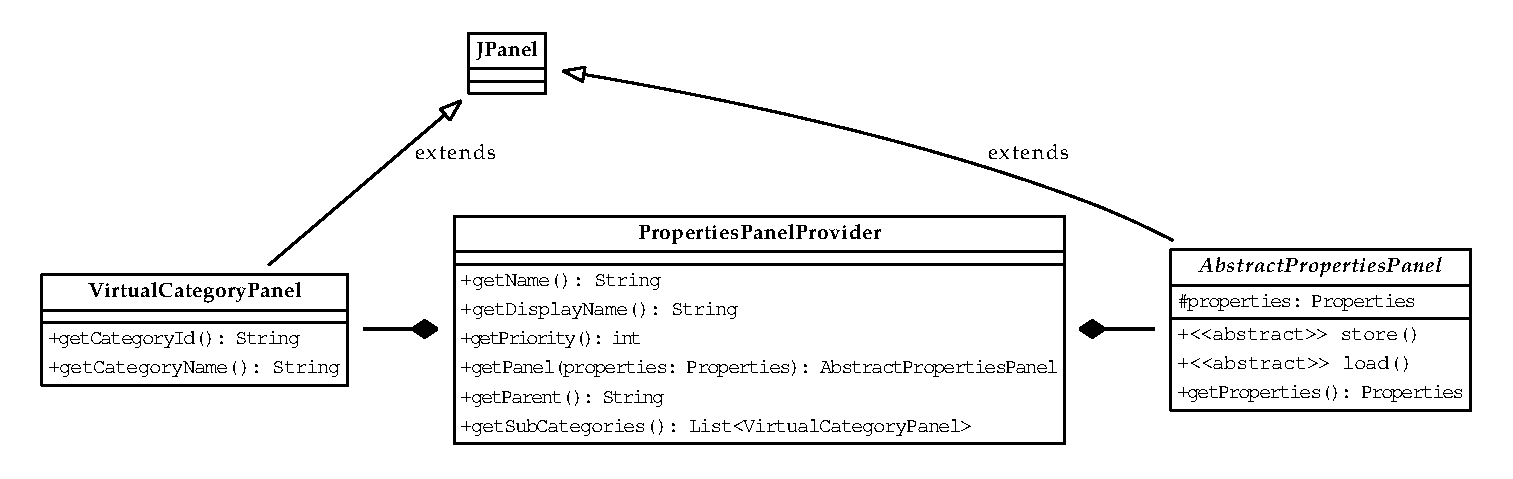
\includegraphics[scale=\myscale]{uml_properties}
	\caption{Class diagram for the custom jInfer project properties category.} \label{uml-properties}
\end{figure}


\subsection{Project wizard}

This section describes the ability of jInfer to create a new jInfer project through a \emph{new project} wizard. This wizard contains two steps, where first is a standard one with project name and location selection, and the second is the selection of Initial Grammar Generator, Simplifier and Schema Generator modules which will be used in inference for this newly created project. New project creation process can be finished in the first step, in which case the default modules will be used for the inference. After finishing the wizard, new jInfer project is created with chosen name in the chosen location. It is important to notice that package \code{cz.\.cuni.\.mff.\.ksi.\.jinfer.\.projecttype} contains \code{JInferTemplateProject.zip} file, in which the default folder structure of a jInfer project is stored. The content of this zip is copied into location defined in the wizard. For more information on how to create a new project wizard, please refer to \cite{project_sample}.\\

All classes responsible for creation of this wizard are in \code{cz.\.cuni.\.mff.\.ksi.\.jinfer.\.projecttype.\.sample} package. It contains \code{JinferTemplateWizardIterator} class defining the number of steps in the wizard and creates a panel for each of these steps. Each step is represented by a class implementing \code{WizardDescriptor.Panel} interface, which creates a step panel and validates its data inserted by the user. Finally there is a class extending \code{JPanel} containing components of the first step.

\subsection{Preferences}\label{pref}

A jInfer project has its own properties category in the project properties window called \emph{Miscellaneous}. This is implemented by \code{ProjectPropertiesPanelProvider} and \code{ProjectPropertiesPanel} classes. In this category, two properties can be set. First property is default \emph{input file} folder to which an unknown input file is inserted (its extension is not defined by any \code{Processor} registered in jInfer). Second property is a global \emph{log} level, which defines the minimum level of messages that will be displayed in jInfer output window. If a module has its own \emph{log} level setting, global settings are overridden by it.


\subsection{RunningProject utility class}\label{running-project}

This section describes \code{RunningProject} utility class, which is not part of the \jmodule{ProjectType} module, but is closely related to it. This class can be found in a \code{cz.\.cuni.\.mff.\.ksi.\.jinfer.\.base.\.utils} package in the \jmodule{Base} module. The main purpose of this class is to allow all jInfer \jmodule{module}s to access the \code{JInferProject} instance of the actual running inference. Notice that in jInfer application only one running inference is allowed at a time.\\

\noindent \code{RunningProject} class implements these methods:
\begin{itemize}
	\item \code{setActiveProject()} - Setter of the \code{JInferProject} instance of a running project, which sets the \code{JInferProject} instance if no other inference is running (no other \code{JInferProject} instance is already set). Returns \code{boolean} value, based on whether the setting was successful.
	\item \code{removeActiveProject()} - Removes the \code{JInferProject} instance if some inference is running.
	\item \code{getActiveProject()} - Getter of the \code{JInferProject} instance of a running project.
	\item \code{isActiveProject()} - Checks if some inference is running (the \code{JInferProject} instance is set).
	\item \code{getActiveProjectProps()} - Gets the \code{Properties} instance from the actual running inference (\code{Properties} instance is part of the \code{JInferProject} instace). If no project is running at the moment, an empty \code{Properties} instance is returned - this allows the JUnit tests to run with default settings.
	\item \code{getNextModuleCaps()} - Getter of capabilities of the next module in the inference chain.
	\item \code{setNextModuleCaps()} - Getter of capabilities of the next module in the inference chain.
\end{itemize}



\nocite{*}
\newpage
\bibliographystyle{alpha}
\bibliography{literature}

\end{document}
